\chapter*{System Memory}
\addcontentsline{toc}{chapter}{System Memory}


\section*{Virtual Address Space}
\addcontentsline{toc}{section}{Virtual Address Space}

Twin-64 features a 52-bit virtual address range. The address range is organized into a 20-bit segment identifier and a 32-bit offset into that segment. The following figure shows the virtual address and how the segment is selected. 

\begin{figure}[H]
\begin{center}
\begin{tikzpicture}[scale=0.9, transform shape]
        
  	\draw[help lines, gray!70, dashed] (0,0) grid(16,15);
        
    \node[  tsRectangle, 
                minimum width=12cm,
                minimum height=1cm,
                fill=white!50] (blocks) at (6,13) { };
                
  	\draw[-] (6,12.5) -- (6, 13.5);
    \draw[-] (2,12.5) -- (2, 13.5);
    
    \node at (11.75,13.75) {0};
	\node at (6.25,13.75) {31};
	\node at (5.75,13.75) {32};
	\node at (2.25,13.75) {51};
	\node at (1.75,13.75) {52};
	\node at (0.25,13.75) {63};           	
    \node at (1,13) {0};
    \node at (4,13) {segId};
    \node at (9,13) {offset};
    	        
    \def\leftofs{9}
	\foreach \i in {0,...,3} {
  		\pgfmathsetmacro\x{ - \i  + \leftofs}
  		\pgfmathsetmacro\y{\i }
  		\draw[tsRectangle, fill=white] (\x,\y) rectangle ++( 6, 8);
	}
		
	\draw[->, thick] (9,12.5) -- (9,11);
	\draw[->, thick] (4,12.5) -- (4,7) -- (5.75,7);
		
	\node at (\leftofs, 7) {Segment};
		
\end{tikzpicture}
\end{center}
\caption{Virtual Memory Address Range}
\label{fig:Virtual Memory Address Range}
\end{figure}

A virtual address to be translated to a physical address. For address translation purposes, the virtual address range can also be seen as a set of virtual pages. The architected page size is 16Kb. A virtual page number is a 38-bit page number with a 14-bit offset into that page. 

\section*{Physical Address Space}
\addcontentsline{toc}{section}{Physical Address Space}

Twin-64 architecture features a 36-bit physical memory address range which allows a maximum physical memory of up to 64 GBytes.  

\begin{figure}[ht]
\begin{center}
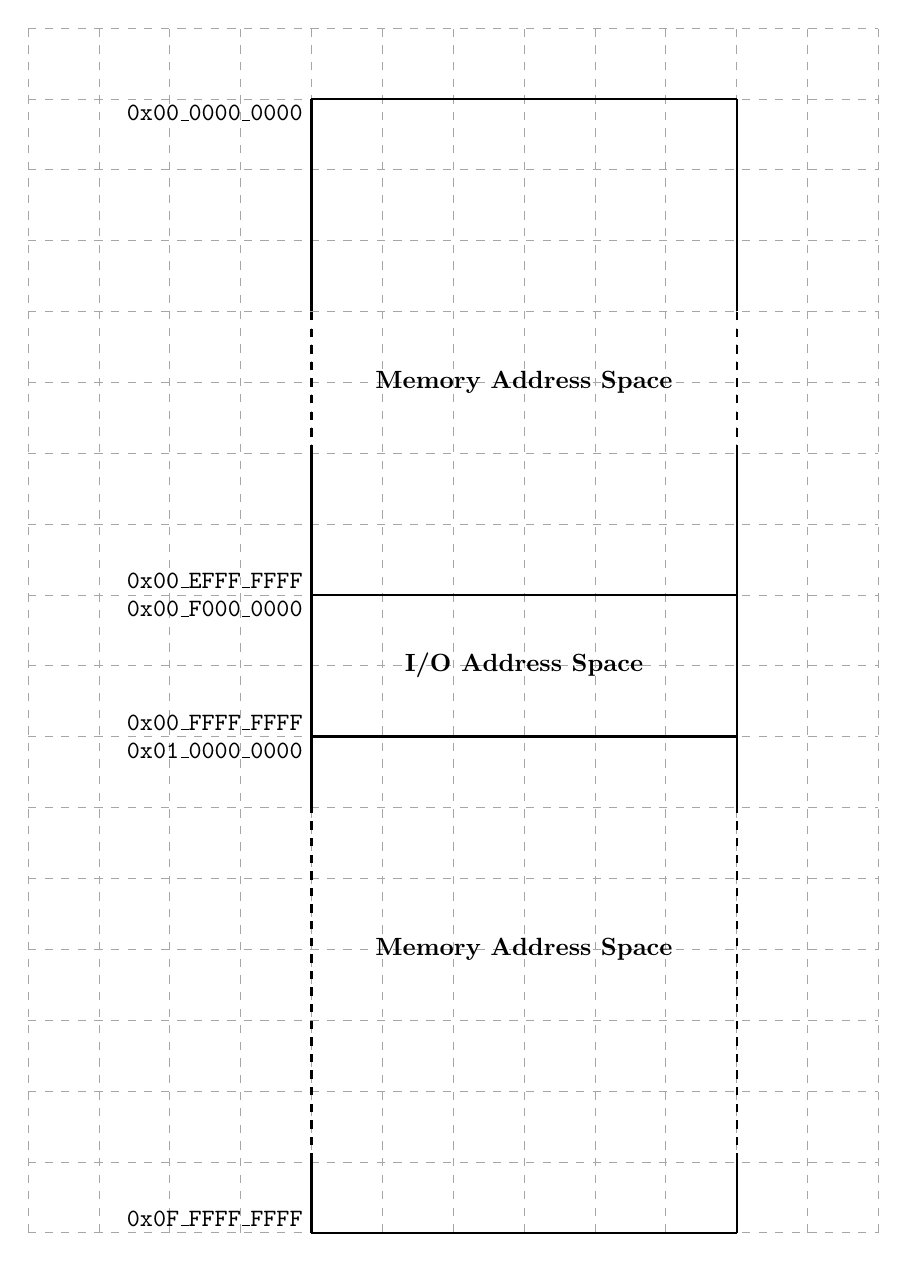
\begin{tikzpicture}[scale=0.9, transform shape]
        
  	\draw[help lines, gray!70, dashed] (0,0) grid(12,17);

	% Rectangle dimensions
	\def\width{6}
	\def\leftofs{4}
	\def\rightofs{\leftofs + \width}

	% Left side
	\draw[thick] (\leftofs, 0) -- (\leftofs, 1);
	\draw[thick, dashed] (\leftofs, 1) -- (\leftofs, 6); 
	\draw[thick] (\leftofs, 6) -- (\leftofs, 11);
	\draw[thick, dashed] (\leftofs, 11) -- (\leftofs, 13); 	
	\draw[thick] (\leftofs, 13) -- (\leftofs, 16);

	% Right side
	\draw[thick] (\rightofs, 0) -- (\rightofs, 1);
	\draw[thick, dashed] (\rightofs, 1) -- (\rightofs, 6); 
	\draw[thick] (\rightofs, 6) -- (\rightofs, 11);
	\draw[thick, dashed] (\rightofs, 11) -- (\rightofs, 13); 	
	\draw[thick] (\rightofs, 13) -- (\rightofs, 16);
		
	% Edges
	\draw[thick] (\leftofs, 0) -- (\rightofs, 0); 
	\draw[thick] (\leftofs, 7) -- (\rightofs, 7); 
	\draw[thick] (\leftofs, 9) -- (\rightofs, 9);
	\draw[thick] (\leftofs, 16) -- (\rightofs, 16);
	
	% Labels 
	\node[left] at (\leftofs, 16 - 0.2) {\texttt{0x00\_0000\_0000}};
	\node[left] at (\leftofs, 9 + 0.2) {\texttt{0x00\_EFFF\_FFFF}};
	\node[left] at (\leftofs, 9 - 0.2) {\texttt{0x00\_F000\_0000}};
	\node[left] at (\leftofs, 7 + 0.2) {\texttt{0x00\_FFFF\_FFFF}};
	\node[left] at (\leftofs, 7 - 0.2) {\texttt{0x01\_0000\_0000}};
	\node[left] at (\leftofs, 0 + 0.2) {\texttt{0x0F\_FFFF\_FFFF}};
		
	\node at (\leftofs + \width / 2, 12) {\textbf{Memory Address Space}};
	\node at (\leftofs + \width / 2, 8) {\textbf{I/O Address Space}};
	\node at (\leftofs + \width / 2, 4) {\textbf{Memory Address Space}};

\end{tikzpicture}
\end{center}
\caption{Physical Memory Address Range}
\label{fig:Physical Memory Address Range}
\end{figure}


Segment Id 0 to 15 directly map to the physical address, without TLB translation and access rights checking. Only privileged mode code can access these segments. Control register zero has a field which encodes the actual memory size installed in a system.


\section*{I/O Address Space}
\addcontentsline{toc}{section}{I/O Address Space}

Twin-64 features memory a mapped I/O architecture. As shown in the overall physical memory layout, the physical memory address range dedicated to I/O modules is located from \texttt{0x00\_F000\_0000} to \texttt{0x00\_FFFF\_FFFF}. The following figure depicts the I/O memory address space ranges in more detail.s

\begin{figure}[H]
\begin{center}
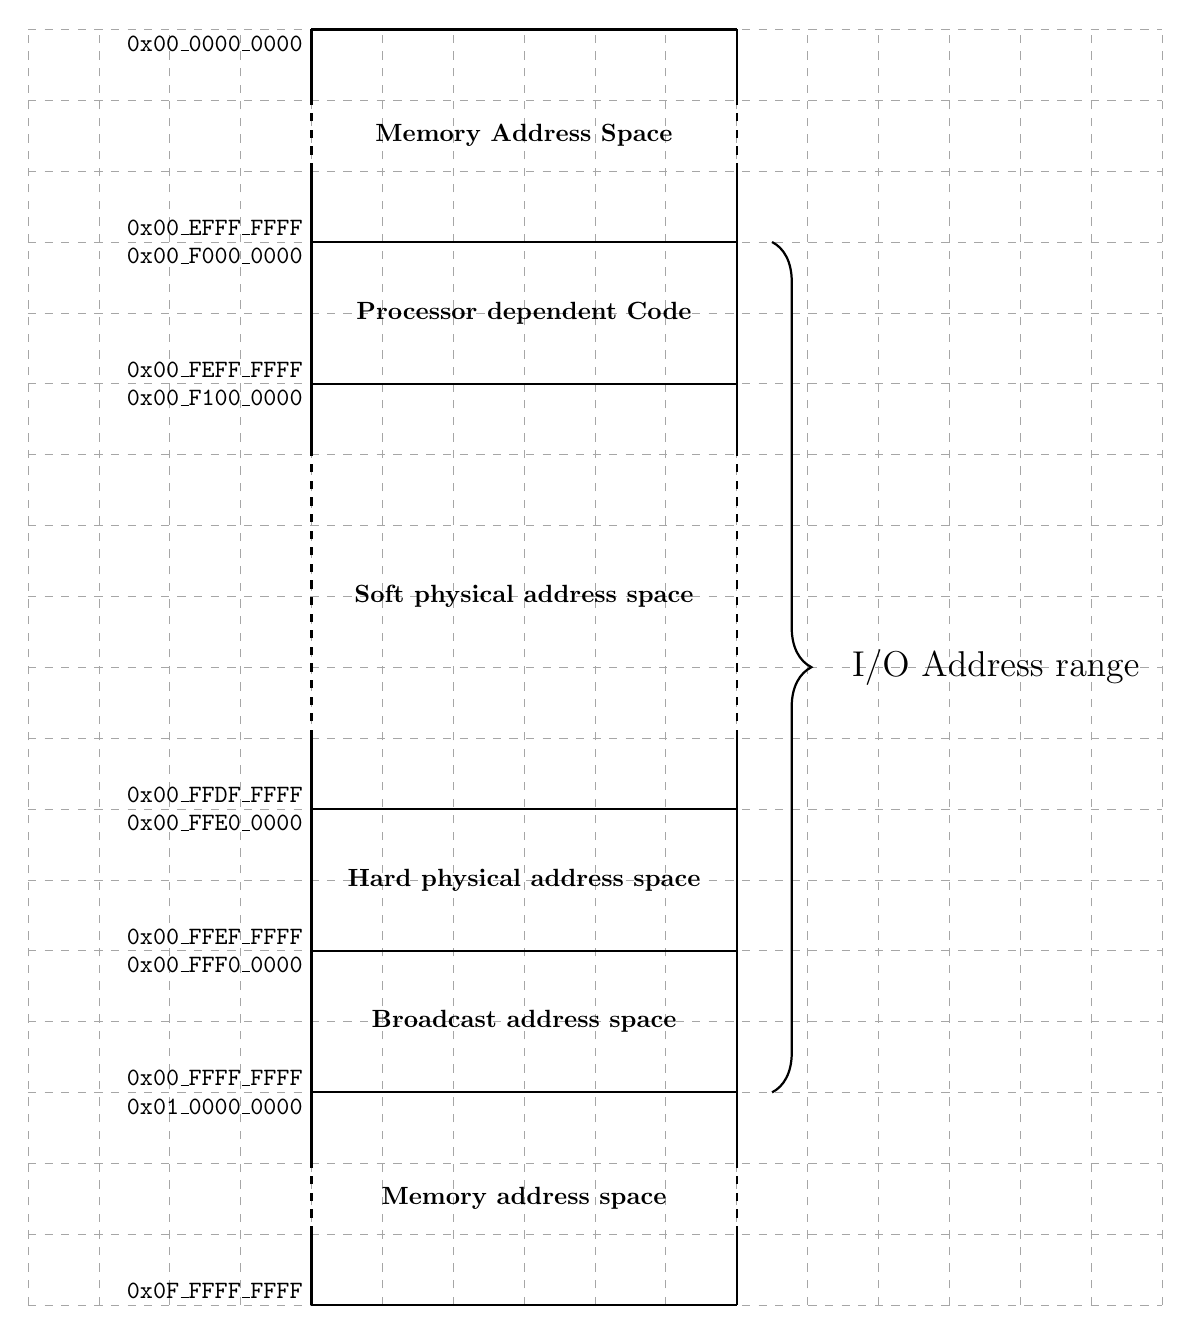
\begin{tikzpicture}[scale=0.9, transform shape]
        
  	\draw[help lines, gray!70, dashed] (0,0) grid(16,18);

	% Rectangle dimensions
	\def\width{6}
	\def\leftofs{4}
	\def\rightofs{\leftofs + \width}

	% Left side
	\draw[thick] (\leftofs, 0) -- (\leftofs, 1); 
	\draw[thick, dashed] (\leftofs, 1) -- (\leftofs, 2);
	\draw[thick] (\leftofs, 2) -- (\leftofs, 8); 
	\draw[thick, dashed] (\leftofs, 8) -- (\leftofs, 12);
	\draw[thick] (\leftofs, 12) -- (\leftofs, 16);
	\draw[thick, dashed] (\leftofs, 16) -- (\leftofs, 17);
	\draw[thick] (\leftofs, 17) -- (\leftofs, 18);

	% Right side
	\draw[thick] (\rightofs, 0) -- (\rightofs, 1); 
	\draw[thick, dashed] (\rightofs, 1) -- (\rightofs, 2);
	\draw[thick] (\rightofs, 2) -- (\rightofs, 8); 
	\draw[thick, dashed] (\rightofs, 8) -- (\rightofs, 12);
	\draw[thick] (\rightofs, 12) -- (\rightofs, 16); 	
	\draw[thick, dashed] (\rightofs, 16) -- (\rightofs, 17);
	\draw[thick] (\rightofs, 17) -- (\rightofs, 18); 
		
	% Edges
	\draw[thick] (\leftofs, 0) -- (\rightofs, 0); 
	\draw[thick] (\leftofs, 3) -- (\rightofs, 3); 
	\draw[thick] (\leftofs, 5) -- (\rightofs, 5); 
	\draw[thick] (\leftofs, 7) -- (\rightofs, 7);
	\draw[thick] (\leftofs, 13) -- (\rightofs, 13);
	\draw[thick] (\leftofs, 15) -- (\rightofs, 15);
	\draw[thick] (\leftofs, 18) -- (\rightofs, 18);
	
	% Labels 
	\node[left] at (\leftofs, 18 - 0.2) {\texttt{0x00\_0000\_0000}};
	\node[left] at (\leftofs, 15 + 0.2) {\texttt{0x00\_EFFF\_FFFF}};
	\node[left] at (\leftofs, 15 - 0.2) {\texttt{0x00\_F000\_0000}};
	\node[left] at (\leftofs, 13 + 0.2) {\texttt{0x00\_FEFF\_FFFF}};
	\node[left] at (\leftofs, 13 - 0.2) {\texttt{0x00\_F100\_0000}};
	\node[left] at (\leftofs, 7 + 0.2) {\texttt{0x00\_FFDF\_FFFF}};
	\node[left] at (\leftofs, 7 - 0.2) {\texttt{0x00\_FFE0\_0000}};
	\node[left] at (\leftofs, 5 + 0.2) {\texttt{0x00\_FFEF\_FFFF}};
	\node[left] at (\leftofs, 5 - 0.2) {\texttt{0x00\_FFF0\_0000}};
	\node[left] at (\leftofs, 3 + 0.2) {\texttt{0x00\_FFFF\_FFFF}};
	\node[left] at (\leftofs, 3 - 0.2) {\texttt{0x01\_0000\_0000}};
	\node[left] at (\leftofs, 0 + 0.2) {\texttt{0x0F\_FFFF\_FFFF}};
		
	\node at (\leftofs + \width / 2, 16.5) {\textbf{Memory Address Space}};
	\node at (\leftofs + \width / 2, 14) {\textbf{Processor dependent Code}};
	\node at (\leftofs + \width / 2, 10) {\textbf{Soft physical address space}};
	\node at (\leftofs + \width / 2, 6) {\textbf{Hard physical address space}};
	\node at (\leftofs + \width / 2, 4) {\textbf{Broadcast address space}};
	\node at (\leftofs + \width / 2, 1.5) {\textbf{Memory address space}};
	
	% bracket
	\draw[thick]  [decorate, decoration={brace, amplitude=0.5cm, mirror}] (\rightofs + 0.5,3) -- (\rightofs + 0.5,15)
	node[midway, right=1cm, anchor=west]{\Large I/O Address range};
	

\end{tikzpicture}
\end{center}
\caption{I/O Memory Address Range}
\label{fig:I/O Memory Address Range}
\end{figure}

The I/O address range is a 256Mbyte area in the first 4 Gbyte segment, i.e.segment 0. The area is divided into several ranges. The first range contains the processor dependent code. There is a set of library functions to manage the processor itself but also provide low-level primitives for the boot process and the operating system. 

The \textbf{hard physical address} range contains a I/O page for each I/O modules installed. There room for 64 I/O modules.

The \textbf{broadcast address} range mirrors the hard physical address range. However, a write to these locations is a write operation to which all I/O modules will react.

The \textbf{soft physical address} range is an area where space is allocated to an I/O module. The I/O module reacts to a memory access operation in its configured soft physical address range.
